\documentclass[12pt,xcolor=x11names]{beamer}
\usetheme{default}
\usecolortheme{seahorse}
\usecolortheme{rose}
\usecolortheme[named=black]{structure}

\usepackage{listings}
\renewcommand*\thelstnumber{\oldstylenums{\the\value{lstnumber}}}
\lstset{
    language=C,
    basicstyle=\footnotesize\ttfamily,
    showstringspaces=false,
    numbers=left,
    numberstyle=\tiny\color{gray},
    keywordstyle=\color{blue}
}

\usepackage{caption}
\usepackage{subcaption}

\title{Seven Deadly Sins of Programming}
\subtitle{}
\author{Mark Simpson \\ \texttt{verdammelt@gmail.com}}
\institute{Angst Programming IG}
\date{\today}

\begin{document}

\begin{frame}
    \titlepage
\end{frame}

\begin{frame}{In the beginning\ldots}

    In the beginning was the Word and the Word was with God and the Word was
    God.
    \pause
    \lstinputlisting{helloworld.c}
\end{frame}

\begin{frame}{The Garden of Eden}
    \begin{figure}
        \begin{subfigure}[b]{0.3\textwidth}
            \centering 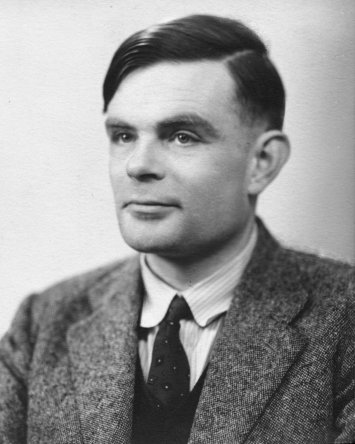
\includegraphics[height=4cm]{images/turing.jpg}
            \caption{Adam}
        \end{subfigure} 
        ~
        \begin{subfigure}[b]{0.3\textwidth}
            \centering 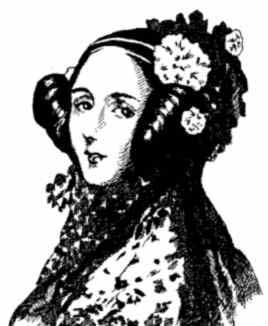
\includegraphics[height=4cm]{images/lovelace.jpg}
            \caption{Eve}
        \end{subfigure}
    \end{figure}
\end{frame}

\begin{frame}{The First Commit}
    \begin{figure}
        \centering 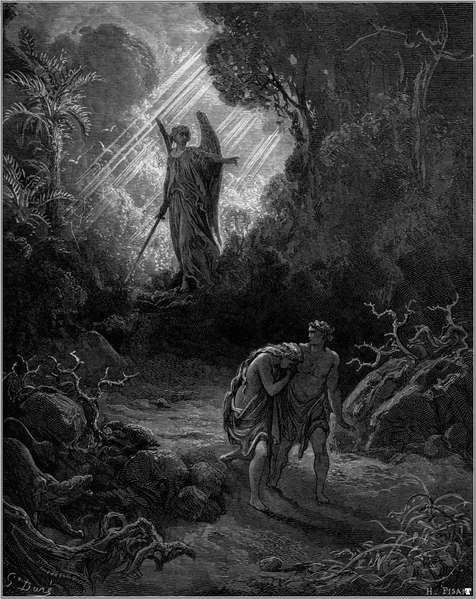
\includegraphics[height=0.75\textheight]{images/castout.png}
    \end{figure}
\end{frame}

\begin{frame}{Luxuria}
    \begin{figure}
        \centering 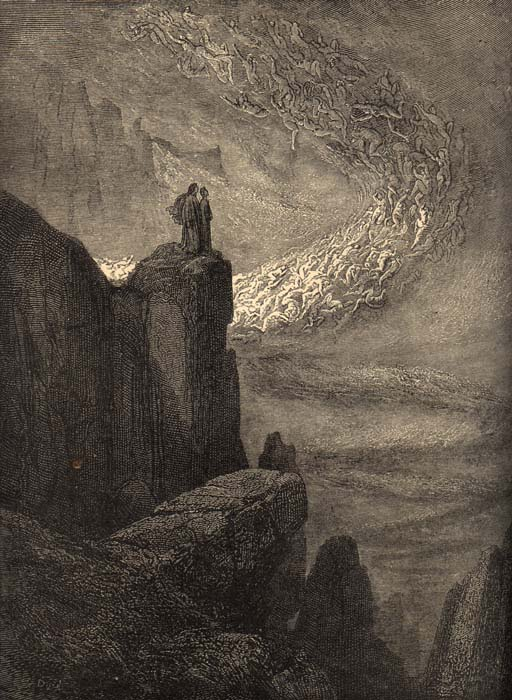
\includegraphics[height=0.75\textheight]{images/lust.jpg}
    \end{figure}
\end{frame}
\begin{frame}{Lust}
    \begin{itemize}
        \item Ooh shiny!
    \end{itemize}
\end{frame}

\begin{frame}{Gula}
    \begin{figure}
        \centering 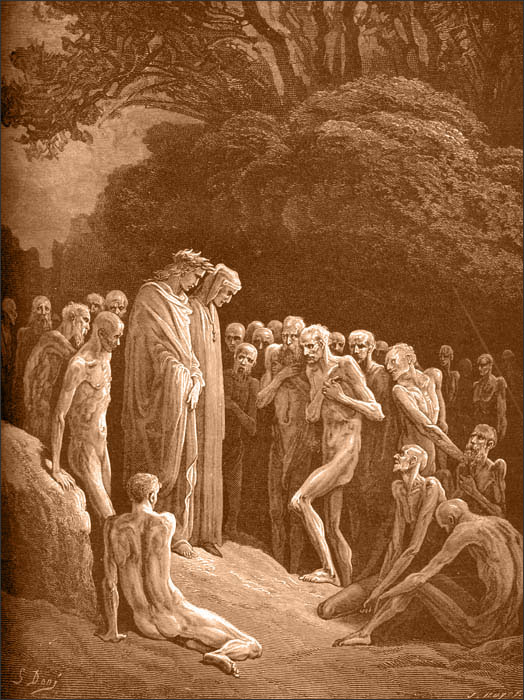
\includegraphics[height=0.75\textheight]{images/gluttony.jpg}
    \end{figure}
\end{frame}
\begin{frame}{Gluttony}
    \begin{itemize}
        \item We'll just add that to this class/function - it's not \emph{too} big yet
        \item We'll add this feature \dots
            \pause
        \item and this one \ldots
            \pause
        \item and this one \ldots
    \end{itemize}
\end{frame}

\begin{frame}{Avaritia}
    \begin{figure}
        \centering 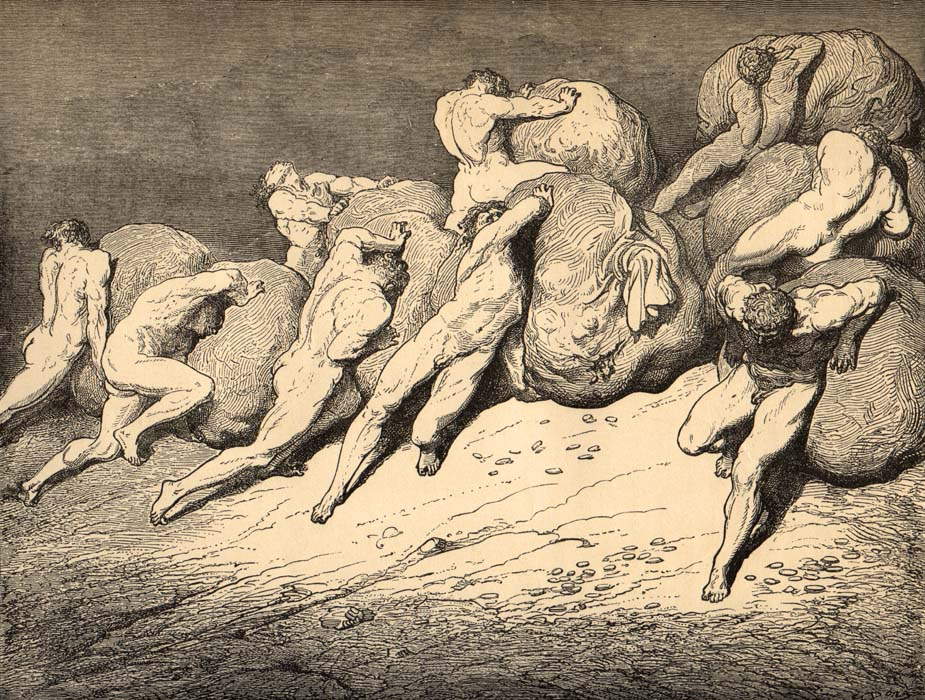
\includegraphics[height=0.75\textheight]{images/greed.jpg}
    \end{figure}
\end{frame}
\begin{frame}{Greed}
    \begin{itemize}
        \item Shh. We can't let the PM know - we don't want this project
            canceled.
        \item No we don't need that \emph{yet}... but we know we'll need it.
        \item We'll use the Composite-Observer-Strategy pattern, because that
            is the way \emph{real} apps are designed.
        \item Certified Scrum Developer -- \emph{nuff said}
    \end{itemize}
\end{frame}

\begin{frame}{Acedia}
    \begin{figure}
        \centering 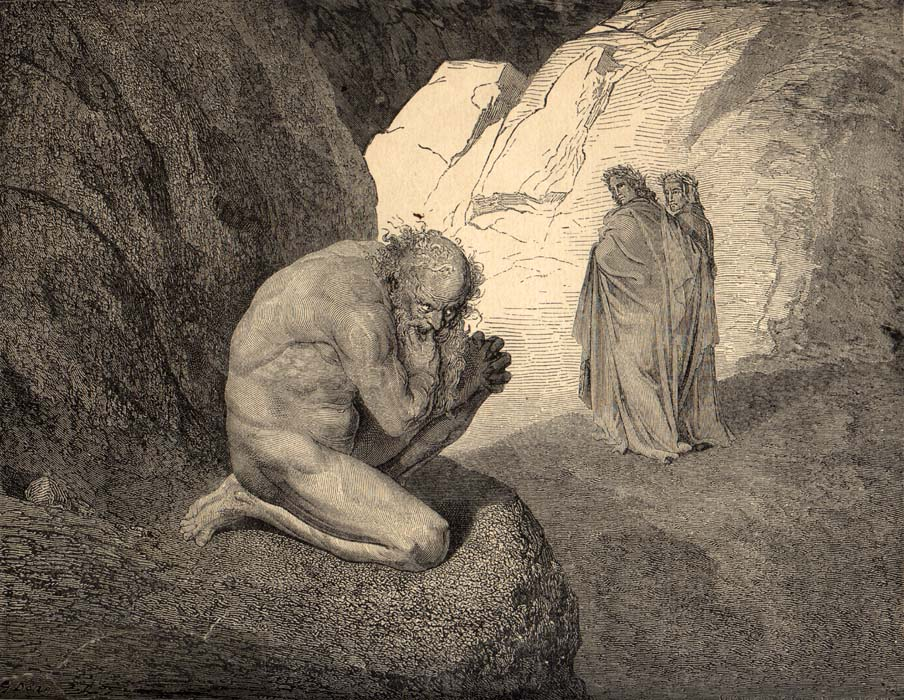
\includegraphics[height=0.75\textheight]{images/sloth.jpg}
    \end{figure}
\end{frame}
\begin{frame}{Sloth}
    \begin{itemize}
        \item I just have to finish this feature, I can clean it up / test it
            later.
        \item Sure the code could be refactored a bit\ldots but that would be
            \emph{Gold Plating}.
    \end{itemize}
\end{frame}

\begin{frame}{Ira}
    \begin{figure}
        \centering 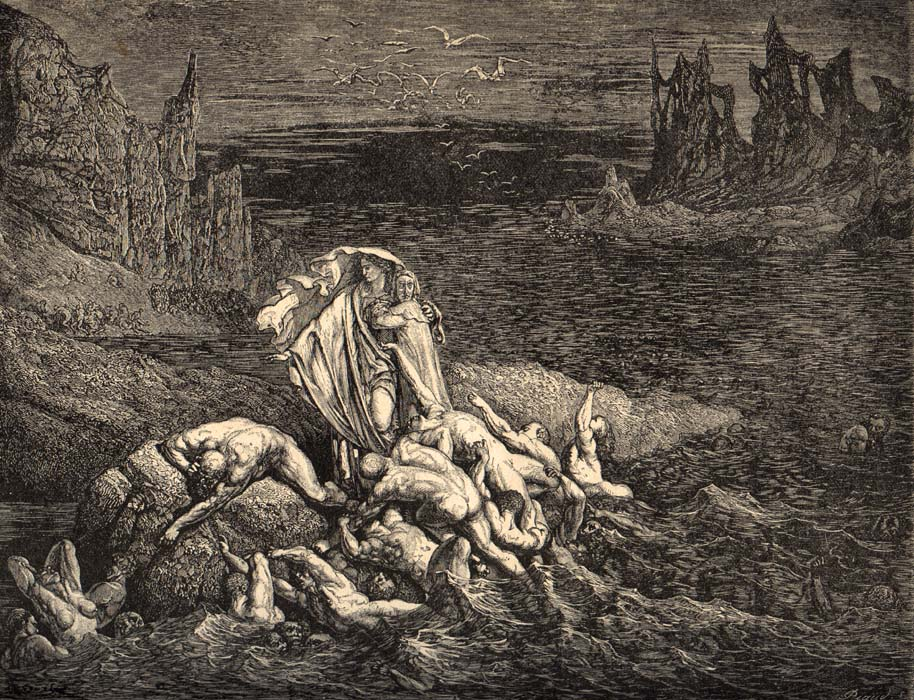
\includegraphics[height=0.75\textheight]{images/wrath.jpg}
    \end{figure}
\end{frame}
\begin{frame}{Wrath}
    \begin{itemize}
        \item We don't do it that way here
        \item Oh we tried that once... didn't work.
        \item WTF why won't this work - maybe if I do this\ldots or this\ldots
        \item TDD is double the work!
    \end{itemize}
\end{frame}

\begin{frame}{Invidia}
    \begin{figure}
        \centering 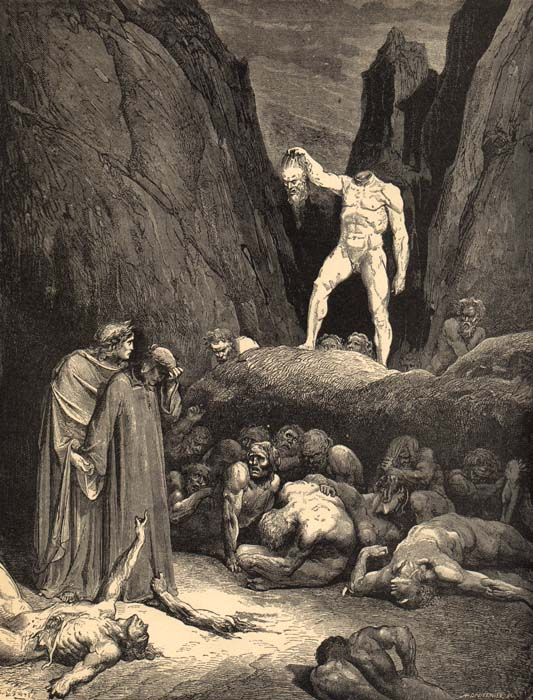
\includegraphics[height=0.75\textheight]{images/envy.jpg}
    \end{figure}
\end{frame}
\begin{frame}{Envy}
    \begin{itemize}
        \item The competitor has this feature - we need it too.
            \pause
        \item \emph{But our app is very different that feature doesn't fit with
            the design.} 
            \pause
        \item Doesn't matter - fit it in there - we must have it!
    \end{itemize}
\end{frame}

\begin{frame}{Superbia}
    \begin{figure}
        \centering 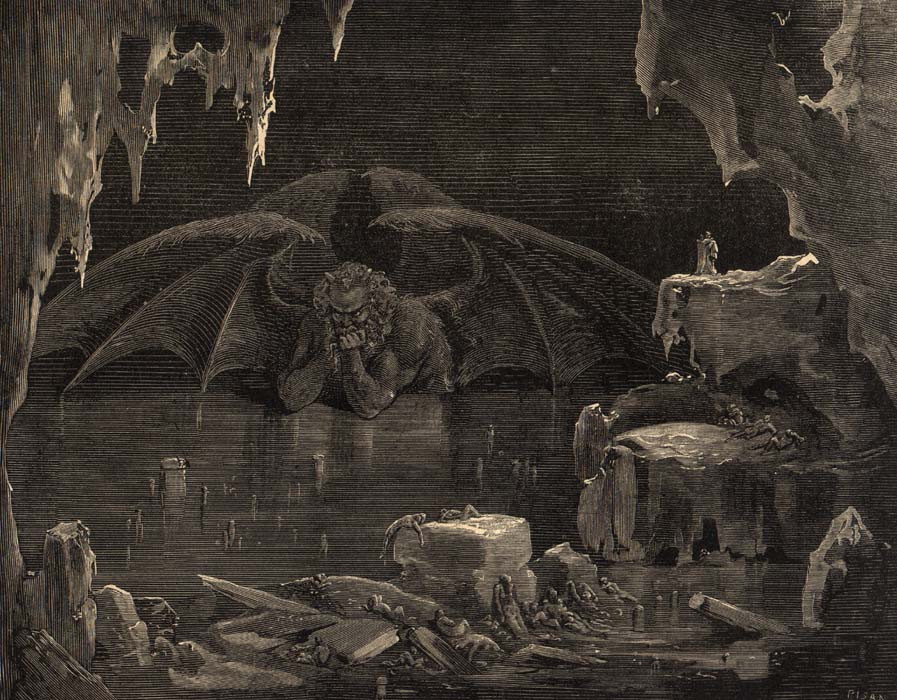
\includegraphics[height=0.75\textheight]{images/pride.jpg}
    \end{figure}
\end{frame}
\begin{frame}{Pride}
    \begin{itemize}
        \item I'm the Architect. My Design is great!
        \item I don't need to test this, I know it is right.
        \item Clever code? This is just a simple triple-pointer to a function
            returning a $\lambda$ that closes over these lexically scoped
            variables and wraps it all in a Monad\ldots
    \end{itemize}
\end{frame}

\begin{frame}{Do not despair\ldots}
    \begin{figure}
        \centering 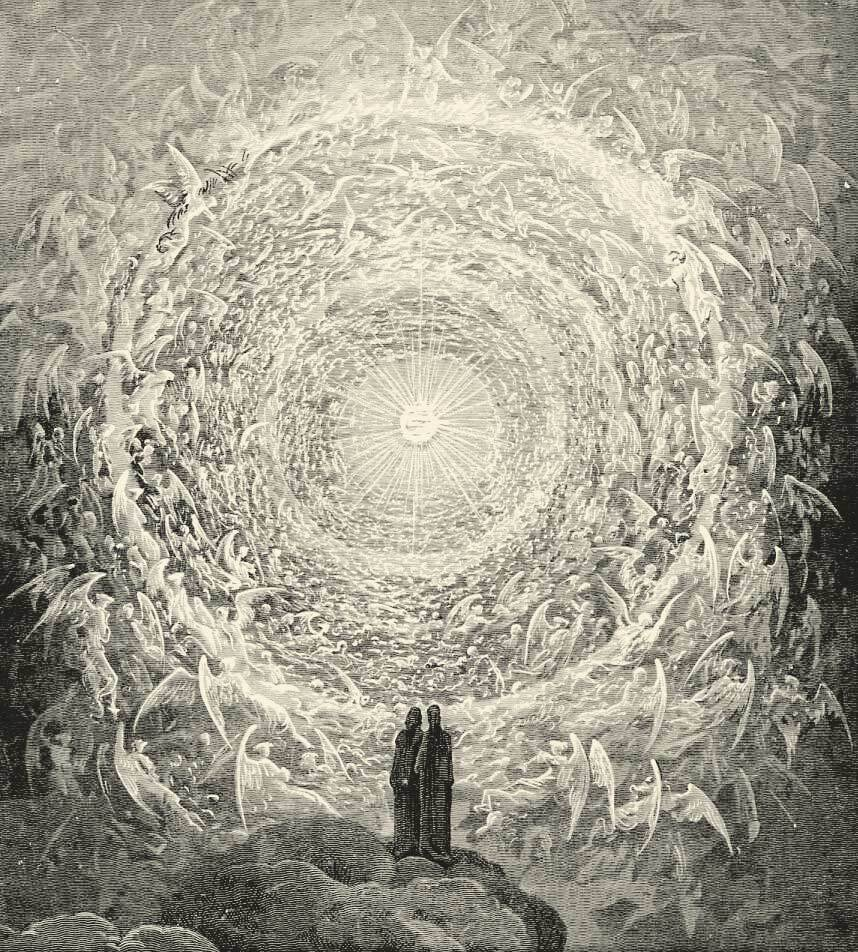
\includegraphics[height=0.75\textheight]{images/hope.jpg}
    \end{figure}
\end{frame}

\begin{frame}{There is hope\ldots}
    Each of the Seven Heavenly Virtues counter one of the Seven Deadly Sins.
    \begin{enumerate}
        \item Castitas / Chastity
        \item Temperantia / Temperance
        \item Caritas / Charity
        \item Industria / Diligence
        \item Patientia / Patience
        \item Humanitas / Kindness
        \item Humilitas / Humility
    \end{enumerate}
\end{frame}

\begin{frame}
    \begin{figure}
        \centering \includegraphics[height=0.75\textheight]{images/emergentdesign.jpg}
    \end{figure}
\end{frame}

\end{document}
